\documentclass{article}

\usepackage{amsmath}
\usepackage{verbatim}
\usepackage{xparse}

\usepackage{tikz}
\usetikzlibrary{calc}
\usetikzlibrary{matrix}
\usetikzlibrary{decorations.pathreplacing,decorations.markings}

\pgfdeclaredecoration{half brace}{brace}
{%
  \state{brace}[width=+\pgfdecoratedremainingdistance, next state=final]
  {%
    \pgfpathmoveto{\pgfpointorigin}%
    \pgfpathcurveto%
    {\pgfqpoint{.15\pgfdecorationsegmentamplitude}{.3\pgfdecorationsegmentamplitude}}%
    {\pgfqpoint{.5\pgfdecorationsegmentamplitude}{.5\pgfdecorationsegmentamplitude}}%
    {\pgfqpoint{\pgfdecorationsegmentamplitude}{.5\pgfdecorationsegmentamplitude}}%
    {%
      \pgftransformxshift{+\pgfdecorationsegmentaspect\pgfdecoratedremainingdistance}%
      \pgfpathlineto{\pgfqpoint{-\pgfdecorationsegmentamplitude}{.5\pgfdecorationsegmentamplitude}}%
      \pgfpathcurveto%
      {\pgfqpoint{-.5\pgfdecorationsegmentamplitude}{.5\pgfdecorationsegmentamplitude}}%
      {\pgfqpoint{-.15\pgfdecorationsegmentamplitude}{.7\pgfdecorationsegmentamplitude}}%
      {\pgfqpoint{0\pgfdecorationsegmentamplitude}{1\pgfdecorationsegmentamplitude}}%
      \pgfpathcurveto%
      {\pgfqpoint{.15\pgfdecorationsegmentamplitude}{.7\pgfdecorationsegmentamplitude}}%
      {\pgfqpoint{.5\pgfdecorationsegmentamplitude}{.5\pgfdecorationsegmentamplitude}}%
      {\pgfqpoint{\pgfdecorationsegmentamplitude}{.5\pgfdecorationsegmentamplitude}}%
    }%
    {%
      \pgftransformxshift{+\pgfdecoratedremainingdistance}%
      \pgfpathlineto{\pgfqpoint{0pt}{.5\pgfdecorationsegmentamplitude}}%
    }%
  }%
  \state{final}{}%
}

\pgfdeclaredecoration{plain brace}{brace}
{%
  \state{brace}[width=+\pgfdecoratedremainingdistance, next state=final]
  {%
    \pgfpathmoveto{\pgfpointorigin}%
    {%
      \pgfpathcurveto%
        {\pgfqpoint{.15\pgfdecorationsegmentamplitude}{.3\pgfdecorationsegmentamplitude}}%
        {\pgfqpoint{.5\pgfdecorationsegmentamplitude}{.5\pgfdecorationsegmentamplitude}}%
        {\pgfqpoint{\pgfdecorationsegmentamplitude}{.5\pgfdecorationsegmentamplitude}}%
    }%
    \pgftransformxshift{+\pgfdecoratedremainingdistance}%
    \pgfpathlineto{\pgfqpoint{-\pgfdecorationsegmentamplitude}{.5\pgfdecorationsegmentamplitude}}%
    {%
      \pgfpathcurveto%
        {\pgfqpoint{-.5\pgfdecorationsegmentamplitude}{.5\pgfdecorationsegmentamplitude}}%
        {\pgfqpoint{-.15\pgfdecorationsegmentamplitude}{.3\pgfdecorationsegmentamplitude}}%
        {\pgfqpoint{0\pgfdecorationsegmentamplitude}{0\pgfdecorationsegmentamplitude}}%
    }%
  }%
  \state{final}{}%
}

\newcommand{\tikzmark}[1]{\tikz[overlay, remember picture] \node (#1) {};}

% tweak these if you wish
\newcommand*{\BraceAmplitude}{0.4em}%
\newcommand*{\BraceAspect}{0.5}%
\newcommand*{\VerticalOffset}{0.5ex}%
\newcommand*{\HorizontalOffset}{0.1em}%
\newcommand*{\TextOffset}{0.66ex}%

\NewDocumentCommand{\AddUnderBrace}{%
	O{}	% #1 = draw options
	O{}	% #2 = optional brace options
	m	% #3 = left tikzmark
	m	% #4 = right tikzmark
	m	% #5 = text to place underbrace
}{%
\begin{tikzpicture}[overlay, remember picture]
	\draw [decoration={plain brace, amplitude=\BraceAmplitude, aspect=\BraceAspect, #2}, decorate, thick, draw=black!80, text=black, #1]
		($ (#4.base) + (\HorizontalOffset,-\VerticalOffset) $) --
		($ (#3.base) + (-\HorizontalOffset,-\VerticalOffset) $)
	node [below=\TextOffset, midway] {#5};
\end{tikzpicture}%
}

\NewDocumentCommand{\AddOverBrace}{%
	O{}	% #1 = draw options
	O{}	% #2 = optional brace options
	m	% #3 = left tikzmark
	m	% #4 = right tikzmark
	m	% #5 = text to place underbrace
}{%
\begin{tikzpicture}[overlay, remember picture]
	\draw [decoration={plain brace, amplitude=\BraceAmplitude, aspect=\BraceAspect, mirror, #2}, decorate, thick, draw=black!80, text=black, #1]
		($ (#4.north) + (\HorizontalOffset,\VerticalOffset+0.25em) $) --
		($ (#3.north) + (-\HorizontalOffset,\VerticalOffset+0.25em) $)
	node [above=\TextOffset, midway] {#5};
\end{tikzpicture}%
}

\begin{document}

\pagestyle{empty}

\[
    \tikzmark{StartBraceAu}\tikzmark{StartBraceAo} \sin^2 \alpha + \cos^2 \theta \tikzmark{EndBraceAu}\tikzmark{EndBraceAo}
    \qquad
    \tikzmark{StartBraceB} \sin^2 \alpha + \cos^2 \theta \tikzmark{EndBraceB}
    \qquad
    \tikzmark{StartBraceC} \sin^2 \alpha + \cos^2 \theta \tikzmark{EndBraceC}
\]

\AddUnderBrace[draw=red, text=blue]{StartBraceAu}{EndBraceAu}{\small below}
\AddOverBrace[draw=red, text=blue]{StartBraceAo}{EndBraceAo}{\small above}

\AddUnderBrace[text=teal][aspect=0.25]{StartBraceB}{EndBraceB}{\small $\mathrm{aspect} = 0.25$}

\AddUnderBrace[text=orange, line cap=round, dash pattern=on 0pt off 1.6\pgflinewidth][aspect=0.75]{StartBraceC}{EndBraceC}{\small $\mathrm{aspect} = 0.75$}

\begin{comment}
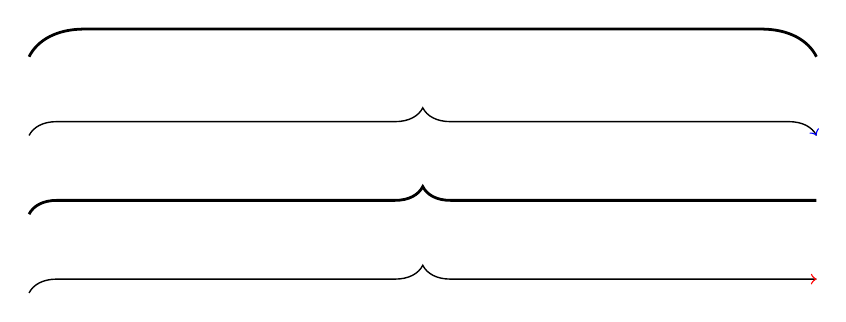
\begin{tikzpicture}
\draw [line width=1pt, decorate, decoration={plain brace,amplitude=20pt}] (0,3) to (10,3);

\draw [line width=0.5pt, postaction=decorate, decoration={markings, mark=at position 1 with {\arrow[blue]{>}}}]
		decorate[decoration={brace, amplitude=10pt}] { (0,2) to (10,2) };
\draw [line width=1pt, decorate, decoration={half brace, amplitude=10pt}] (0,1) to (10,1);
\draw [line width=0.5pt, postaction=decorate, decoration={markings, mark=at position 1 with {\arrow[red]{>}}}]
		decorate[decoration={half brace, amplitude=10pt}] { (0,0) to (10,0) };
\end{tikzpicture}
\end{comment}

\newpage

\tikzstyle{overbrace text style}=[font=\tiny, above, pos=.5, yshift=3mm]
\tikzstyle{overbrace style}=[decorate,decoration={brace,raise=2mm,amplitude=3pt}]
\tikzstyle{underbrace style}=[decorate,decoration={brace,raise=2mm,amplitude=3pt,mirror},color=gray]
\tikzstyle{underbrace text style}=[font=\tiny, below, pos=.5, yshift=-3mm]

\begin{tikzpicture}

    \matrix[name=M1, matrix of nodes, inner sep=0pt, column sep=0pt]{
      \node (schema) [text=red] {http:\vphantom{/}}; & \node (schema-spezifisch) [text=black] {//}; & \node (nutzerinfo) [text=orange] {user:pass\vphantom{/}}; & @ & \node (host) [text=blue] {www.example.com\vphantom{/}}; & : & \node (port) [text=blue!40] {1234\vphantom{/}}; & \node (pfad) [text=red] {/directory/index.php}; & \node (query) [text=purple] {?key=value\vphantom{/}}; & \node (fragment) [text=green] {\#anchor\vphantom{/}};  \\
    };

    \draw [overbrace style] (schema.north west) -- (schema.north east) node [overbrace text style] {Schema};
    \draw [overbrace style] (schema-spezifisch.north west) -- (fragment.north east) node [overbrace text style] {Schema-Spezifisch};
    \draw [underbrace style] (nutzerinfo.south west) -- (nutzerinfo.south east) node [underbrace text style,text=orange] {Nutzerinfo};
    \draw [underbrace style] (host.south west) -- (host.south east) node [underbrace text style,text=blue] {Host};
    \draw [underbrace style] (port.south west) -- (port.south east) node [underbrace text style,text=blue!40,baseline] {Port};
    \draw [underbrace style] (pfad.south west) -- (pfad.south east) node [underbrace text style,text=red] {Pfad};
    \draw [underbrace style] (query.south west) -- (query.south east) node [underbrace text style,text=purple] {Query};
    \draw [underbrace style] (fragment.south west) -- (fragment.south east) node [underbrace text style,text=green] {Fragment};

\end{tikzpicture}

\begin{tikzpicture}

    \matrix[name=M2, matrix of nodes, inner sep=0pt, column sep=0pt]{
      \node (URI) {http:}; & \node (schema) [text=black] {//user:password@domain.com:port/resource?query=foo}; & \node (fragment) {\#fragment};  \\
    };

    \draw [overbrace style] (URI.north west) -- (fragment.north east) node [overbrace text style] {URI};
    \draw [decorate,decoration={brace,raise=6mm,amplitude=3pt,mirror},color=gray] (schema.south west) -- (fragment.south east) node [font=\tiny, below, pos=.5, yshift=-7mm] {Schema};
    \draw [underbrace style] (fragment.south west) -- (fragment.south east) node [underbrace text style] {Fragment};

\end{tikzpicture}

\end{document}
